%
%
%
%
%
%
%




\documentclass{beamer}
\usetheme{Copenhagen}
\usepackage[utf8]{inputenc}


%\usepackage{graphicx}
%\usepackage{subfigure}
%\usepackage{multimedia}
\usepackage{times}  % fonts are up to you
\usepackage{graphics}
\usepackage{amsmath}
\usepackage{media9}
\usepackage{hyperref}
\usepackage{psfrag}
\usepackage{pdfpages}
\usepackage{listings}
%\usepackage[style=authoryear]{biblatex}
%\bibliography{/Users/ali/Library/texmf/bibtex/bib/references}


\setbeamertemplate{bibliography item}[text]
%\usepackage[backend=bibtex, style=authoryear]{biblatex}
%\addbibresource{/Users/ali/Library/texmf/bibtex/bib/references.bib}
\newcommand{\customcite}[1]{\citeauthor{#1}, \citeyear{#1}}
\newcommand\smallFont{\fontsize{8}{7.2}\selectfont}   %Change font size.
\newcommand\mCite[1]{[\cite{#1}, \citetitle{#1}]}  %Prints name and title
\newcommand\FrameText[1]{
\begin{textblock*}{\paperwidth}(0pt,\textheight)
	\vspace{1.0cm}
    \raggedleft \smallFont #1
\end{textblock*}}

%Get rid of ugly copenhagen default symbol for enumerate
\setbeamertemplate{enumerate items}[default]   


% Create code text
% https://tex.stackexchange.com/questions/65291/code-snippet-in-text
\definecolor{codegray}{gray}{0.9}
\newcommand{\code}[1]{\colorbox{codegray}{\texttt{#1}}}



%Information to be included in the title page:
\title{Introduction to Slurm}
\author{Ali Snedden}
\institute{Nationwide Children's Hospital}
\date{April 19, 2019}
 
 
 
\begin{document}
 
\frame{\titlepage}




\begin{frame}
\frametitle{How to Connect}
Windows:
\begin{itemize}
    \item Open PuTTY
    \item Window Session $\Rightarrow$ Host Name field : username@10.70.250.101
    \item Click ``Open" to log in.
    \item Enter password
\end{itemize}

Mac:
\begin{itemize}
    \item Open Terminal (Finder $\Rightarrow$ Utilities $\Rightarrow$ Terminal)
    \item \code{ssh -X username@10.70.250.101}
\end{itemize}

\end{frame}


\begin{frame}
\frametitle{Cluster Architecture}
\begin{picture}(320,250)  %must be related to where it is centered
%\put(0, 70){\includegraphics[height=2.5in]{images/GPFS_File.eps}}
%\setbeamercolor{background canvas}{bg=}
%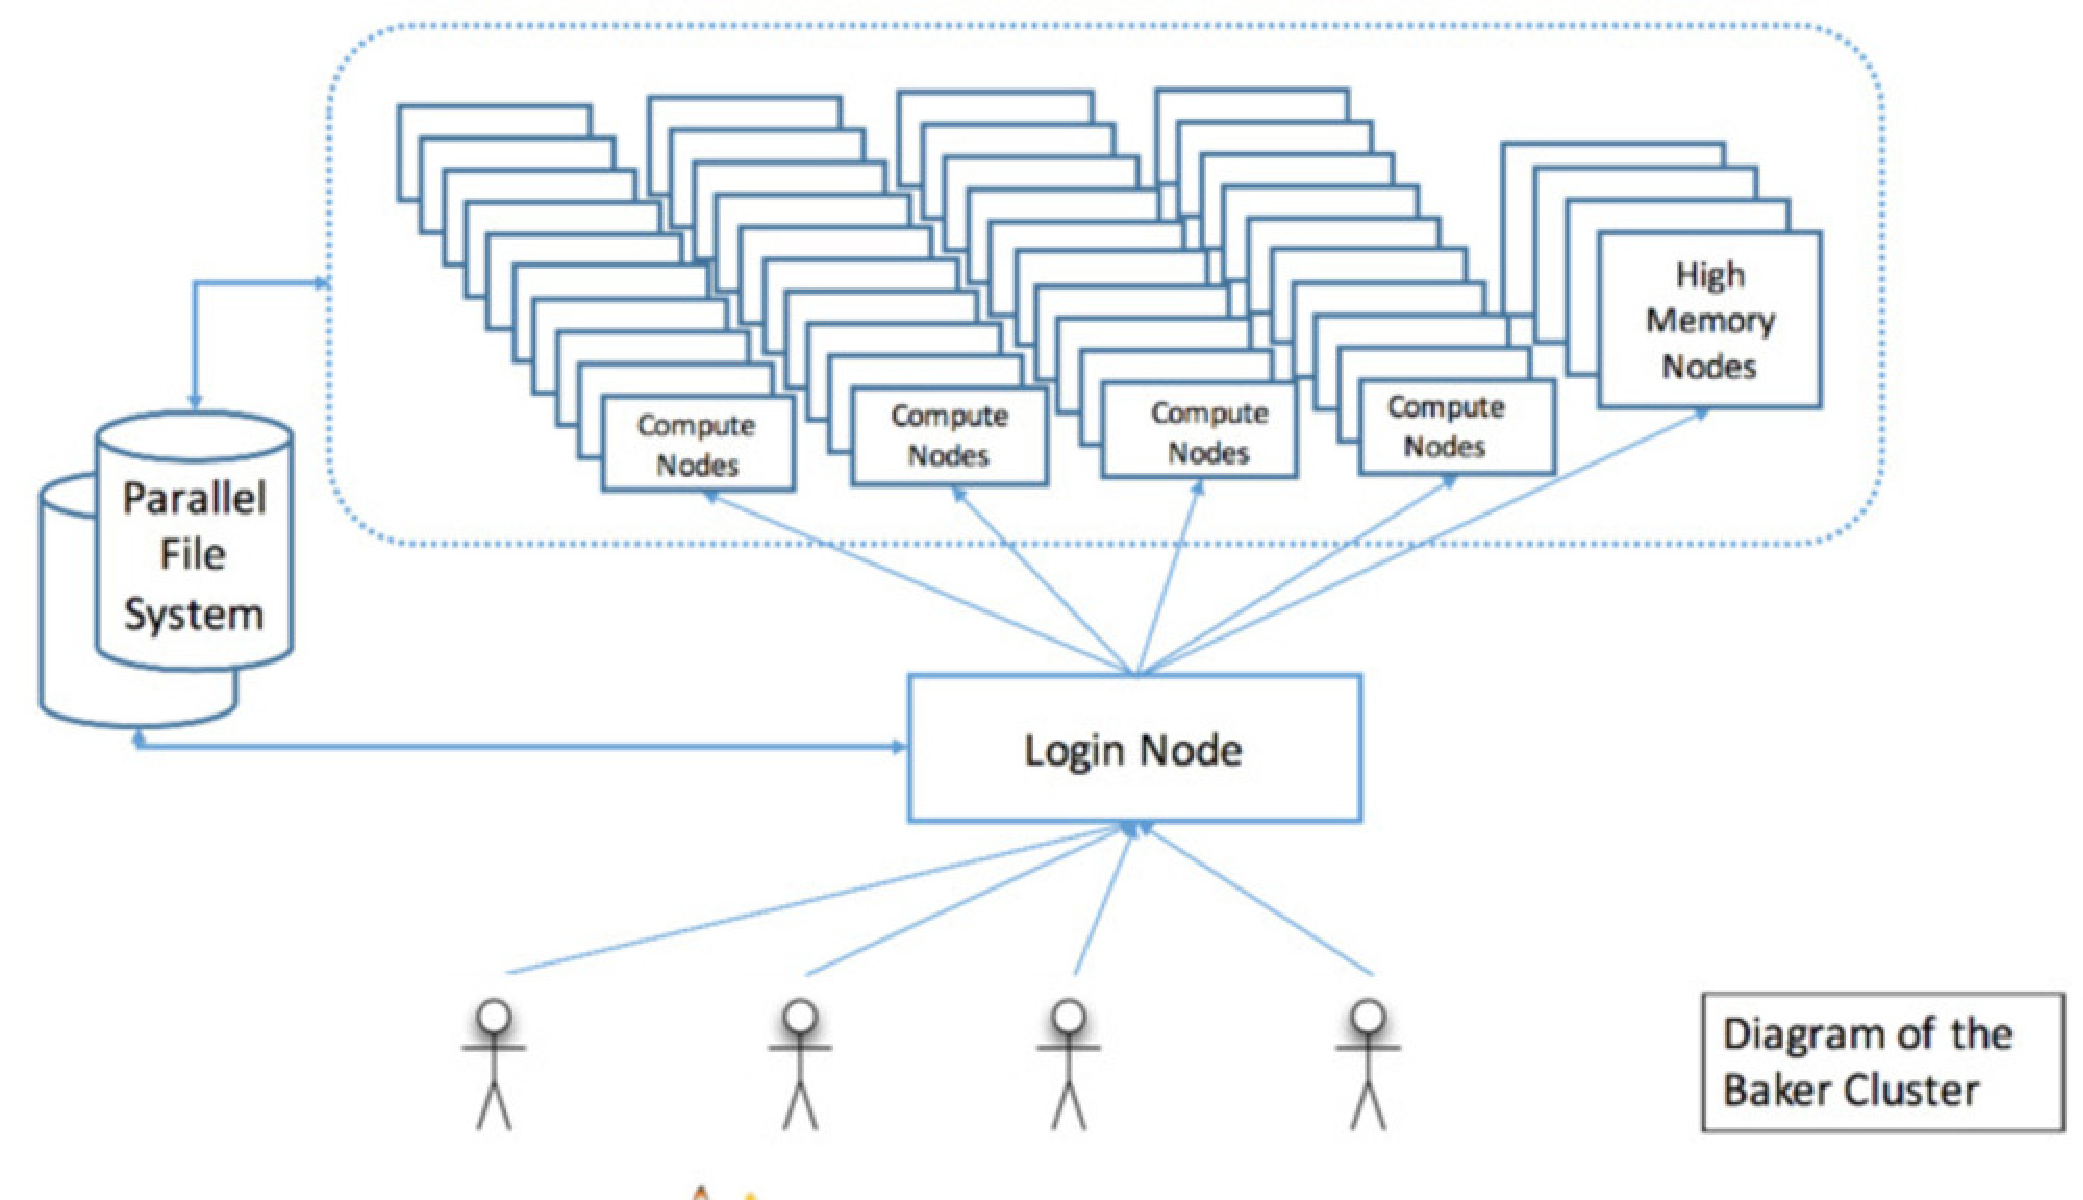
\includepdf{images/GPFS_File-eps-converted-to.pdf}
%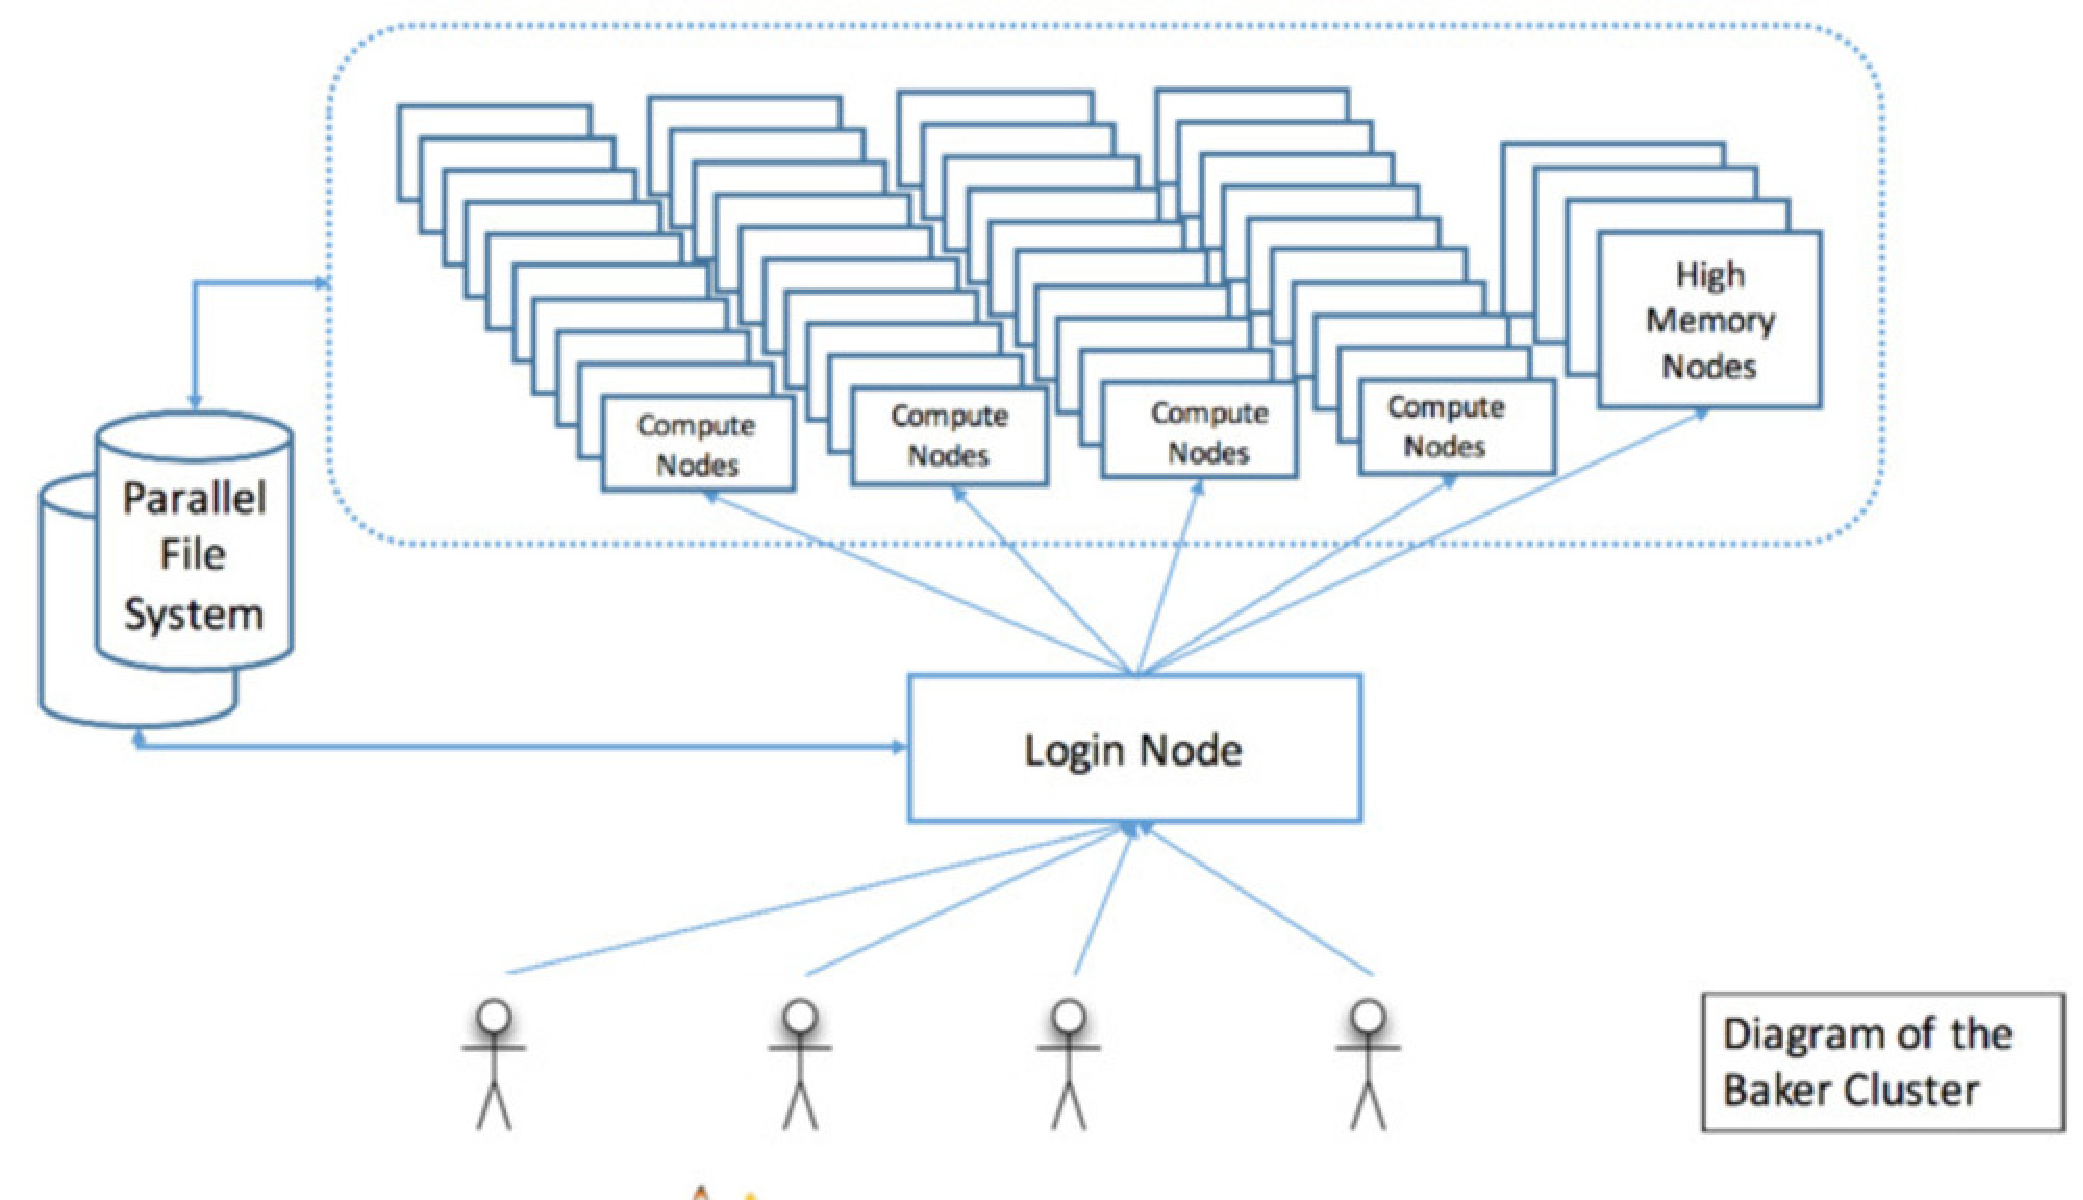
\includepdf{images/GPFS_File-eps-converted-to.pdf}

\put(0, 70){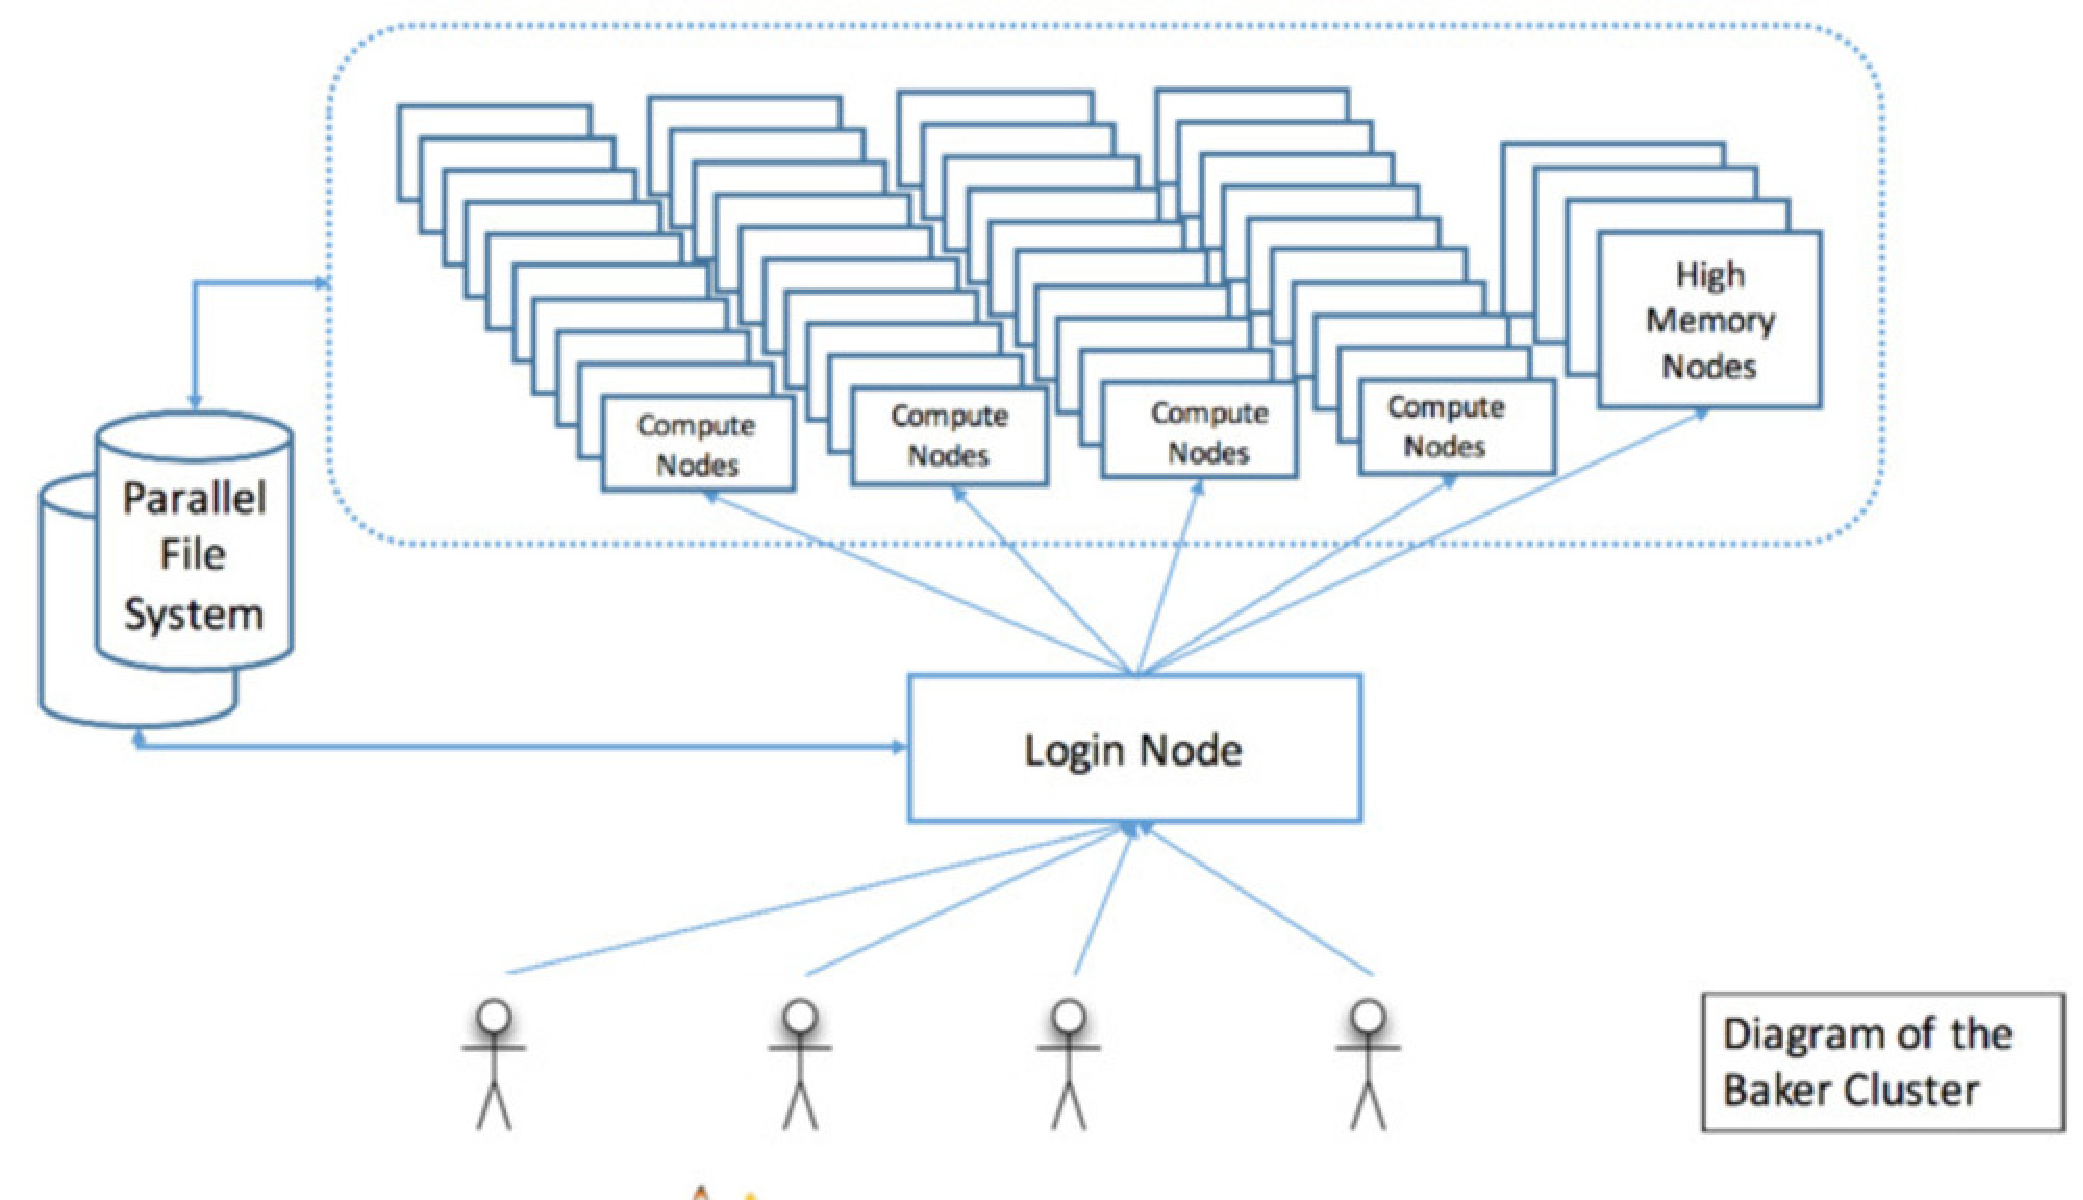
\includegraphics[height=2.5in]{images/GPFS_File-eps-converted-to.pdf}}
\end{picture}
\end{frame}


\begin{frame}
\frametitle{Cluster Architecture}
Type of hardware available
\begin{itemize}
    \item High Memory (himem)
    \begin{enumerate}
        \item 1.5 TB RAM
        \item 48 cores 
        \item Ivy Bridge CPUs - slower memory access
    \end{enumerate}
    \pause 
    \bigskip
    \pause
    \item General Purpose (default)
    \begin{enumerate}
        \item 128 GB RAM
        \item 20 cores 
        \item Haswell - faster memory access
    \end{enumerate}
    \bigskip
    \pause
    \item GPU 
    \begin{enumerate}
        \item 128 GB and 192GB RAM 
        \item 20 cores 
        \item Haswell and Skylake CPUs
        \item NVidia K40, P100 and V100 available
    \end{enumerate}
\end{itemize}
\end{frame}


\begin{frame}
\frametitle{Cluster Architecture}
Storage 
\begin{itemize}
    \item 429 TB of storage available
    \pause
    \item No limits on user storage - be responsible.
          It takes everyone's cooperation to have this nice feature.
    \pause
    \item Not intended for archival or long term storage.
        \begin{enumerate}
              \item Be sure to back up your important data and code elsewhere
              \item If data center goes up in smoke, your research, time and grant money may as well.
        \end{enumerate}
    \pause
    \item PHI permitted
\end{itemize}
\pause
Networking:
\begin{itemize}
    \item 56 Gb/s Infiniband fabric available
\end{itemize}
\end{frame}


\begin{frame}
\frametitle{HPC Concepts}
Parallelization:
\begin{itemize}
    \item Shared memory
        \begin{enumerate}
            \item All memory used is within the same physical computer
            \pause
            \item Often used for 'embarrassingly parallizeable' problems
            \pause 
            \item Protocals 
                \begin{itemize}
                    \item C/Fortran : OpenMP
                    \item R : parapply package
                    \item Python : multiprocessing module
                \end{itemize}
        \end{enumerate}
    
    \pause
    \bigskip
    \item Distributed memory
        \begin{enumerate}
            \item Memory is distributed amongst multiple computers
            \pause
            \item Protocals 
                \begin{itemize}
                    \item C/Fortran : MPI
                    \item Any language : Server-Client model over ports
                \end{itemize}
        \end{enumerate}
\end{itemize}
\end{frame}
 


\begin{frame}
\frametitle{What is Slurm?}
Need method for managing cluster resources.
\bigskip
\begin{itemize}
    \pause
    \item Enter SLURM - A Workload Manager
    \bigskip
    \pause
    \begin{enumerate}
        \item Permits efficient (and fair) utilization of Cluster resources.
        \pause
        \bigskip
        \item This is your interface with the computer cluster
    \end{enumerate}
\end{itemize}
\end{frame}



\begin{frame}
\frametitle{Slurm Concepts}
\begin{itemize}
    \item Job
    \pause 
    \begin{enumerate}
        \item Primary way of requesting resources
        \pause
        \item Composed of one or more Steps
    \end{enumerate}
    \bigskip
    \pause
    \item Step
    \begin{enumerate}
        \item A way of dividing the resources allocated
        \pause
        \item Can be run serially or in parallel within a job
        \pause
        \item Composed of one or more Tasks
    \end{enumerate}
    \bigskip
    \pause
    \item Task
    \begin{enumerate}
        \item Composed of one or more CPUs
    \end{enumerate}
    \bigskip
\end{itemize}
\end{frame}



\begin{frame}
\frametitle{Baker}
A typical job on Baker : 
\bigskip
\begin{itemize}
    \item 1 Node 
    \pause 
    \bigskip
    \pause
    \item 1 Task
    \bigskip
    \pause
    \item Multiple CPUs
    \bigskip
    \pause
\end{itemize}
Complicated jobs may benefit from utilizing multiple steps and tasks, most jobs will not.
\end{frame}



\begin{frame}
\frametitle{How to use Slurm?}
\begin{itemize}
    \item \code{sbatch} - Bash script
    \bigskip
    \pause
    \item \code{salloc} - Interactive sessions
    \bigskip
    \pause
    \item \code{srun-x11} - Interactive sessions - with x11 forwarding
    \bigskip
\end{itemize}
\end{frame}



\begin{frame}
\frametitle{sbatch}
Examples of Usage:
\bigskip
\begin{itemize}
    \item \code{sbatch myscript.sh}
    \bigskip
    \pause
    \item \code{sbatch --cpus-per-task=20 myscript.sh}
    \bigskip
    \pause
    \begin{enumerate}
        \item NOTE : specifying 20 cores, will not magically make your script use 20 cores.
                     You will need to specify that within your shell script \code{myscript.sh}
    \end{enumerate}
    \item \code{sbatch --gres=gpu:p100 myscript.sh}
    \bigskip
\end{itemize}
\end{frame}



\begin{frame}
\frametitle{sbatch}
Two ways to pass arguments to sbatch
\smallskip
\begin{itemize}
    \item Command line
        \smallskip
        \begin{enumerate}
            \item E.g. \code{sbatch OPTIONS myscript.sh}
            \pause
            \smallskip
            \item Popular \code{OPTIONS}
            \begin{itemize}
                \item \code{--cpus-per-task=} 
                \smallskip
                \item \code{--partition=} \code{himem}
                \pause
                \smallskip
                \item \code{--gres=} \code{gpu:p100}, \code{gpu:k40}, \code{gpu:v100}
            \end{itemize}
            \pause
            \smallskip
            \item Preempts options set in bash script
        \end{enumerate}
        \smallskip

    \pause
    \item In Bash Script, \code{myscript.sh}
        \smallskip
        \begin{enumerate}
            \item Popular \code{OPTIONS}
            \begin{itemize}
                \item \code{\#SBATCH --cpus-per-task=} 
                \pause
                \smallskip
                \item \code{\#SBATCH --partition=} \code{himem}
                \pause
                \smallskip
                \item \code{\#SBATCH --gres=} \code{gpu:p100}, \code{gpu:k40}, \code{gpu:v100}
            \end{itemize}
        \end{enumerate}
\end{itemize}
\end{frame}



\begin{frame}[fragile]
\frametitle{sbatch}
Example \code{myscript.sh}: 
\begin{lstlisting}[backgroundcolor = \color{codegray}, language = Bash]
    #!/bin/bash
    #SBATCH --cpus-per-task=10
    set -e
    echo "Hello World"
    sleep 30
\end{lstlisting}
\bigskip
\bigskip
Submit with \code{sbatch myscript.sh}
\end{frame}


\begin{frame}[fragile]
\frametitle{sbatch}
Output from batch script (\code{slurm-1795906.out}), will have some of the below information (some columns abbreviated for clarity)
\begingroup
\tiny
\begin{lstlisting}[backgroundcolor = \color{codegray}, language = Bash]
Hello World
Job Statistics for 179:
       JobID   User Start End   Elapsed  MaxRSS   TotalCPU State Exit  NodeList ReqTRES
------------ ------ ----- --- --------- ------- ---------- ----- ---- --------- ----------------
         179 aps003 ..... ...  00:00:00          00:00.009 COMPL  0:0    node01  cpu=1,mem=6144M
   179.batch        ..... ...  00:00:00       0  00:00.008 COMPL  0:0    node01
  179.extern        ..... ...  00:00:00       0   00:00:00 COMPL  0:0    node01
CPU Efficiency: 0.00% of 00:00:00 core-walltime
\end{lstlisting}
\endgroup
\end{frame}


\begin{frame}[fragile]
\frametitle{sbatch}
Himem partition example \code{myscript\_himem.sh}: 
\begin{lstlisting}[backgroundcolor = \color{codegray}, language = Bash]
    #!/bin/bash
    #SBATCH --cpus-per-task=2
    #SBATCH --partition=himem
    set -e
    echo "Hello World"
    sleep 30
\end{lstlisting}
\bigskip
\bigskip
Submit with \code{sbatch myscript\_himem.sh}
\end{frame}


\begin{frame}[fragile]
\frametitle{sbatch}
GPU example \code{myscript\_gpu.sh}: 
\begin{lstlisting}[backgroundcolor = \color{codegray}, language = Bash]
    #!/bin/bash
    #SBATCH --cpus-per-task=2
    #SBATCH --gres=gpu:p100
    set -e
    echo "Hello World"
    sleep 30
\end{lstlisting}
\bigskip
\bigskip
Submit with \code{sbatch myscript\_gpu.sh}
\end{frame}



\begin{frame}[fragile]
\frametitle{sbatch}
Broken Example \code{myscript\_broken.sh}: 
\begin{lstlisting}[backgroundcolor = \color{codegray}, language = Bash]
    #!/bin/bash
    #SBATCH --cpus-per-task=2
    #SBATCH --partition=himem
    #SBATCH --mail-user=First.Last@gmail.com
    #SBATCH --mail-type=FAIL,TIME_LIMIT_90
    set -e
    echo "I'm looking in the forbidden location"
    ls /root/
    echo "I never make it here"
\end{lstlisting}
\bigskip
\bigskip
Submit with \code{sbatch myscript\_broken.sh}
\end{frame}



\begin{frame}
\frametitle{salloc}
\code{salloc} - Interactive allocation 
\bigskip
\begin{itemize}
    \item Use when needing to interactively run long processes. E.g.
        \begin{enumerate}
            \item compiling
            \bigskip
            \pause 
            \item developing and testing workflows
            \bigskip
            \pause 
            \item downloading data
            \bigskip
            \pause 
        \end{enumerate}
    \pause
    \pause
    
    \item Example of Running:
    \bigskip
    \begin{enumerate}
        \item \code{salloc --cpus-per-task=2}
        \bigskip
        \item \code{srun  --jobid XXXX --pty bash}
        \pause
        \bigskip
        \item \code{salloc} takes all same command line options as \code{sbatch}
    \end{enumerate}
\end{itemize}
\end{frame}


\begin{frame}
\frametitle{srun-x11}
\code{srun-x11} - Interactive allocations with X11 forwarding
\bigskip
\begin{itemize}
    \item Use when needing graphical processes
        \bigskip
        \begin{enumerate}
            \item GUI editors, e.g. RStudio
            \bigskip
            \pause 
            \item Plotting, e.g. gnuplot, matplotlib
            \bigskip
        \end{enumerate}
    \pause
    \item Example of Running:
    \bigskip
    \begin{enumerate}
        \item \code{srun-x11 --cpus-per-task=2}
        \bigskip
        \pause
        \item Limited to 10h, can change by passing \code{time} option, e.g. \code{srun-x11 --time=2-00:00:00}
    \end{enumerate}
\end{itemize}
\end{frame}


\end{document}
